% This file was created with tikzplotlib v0.10.1.
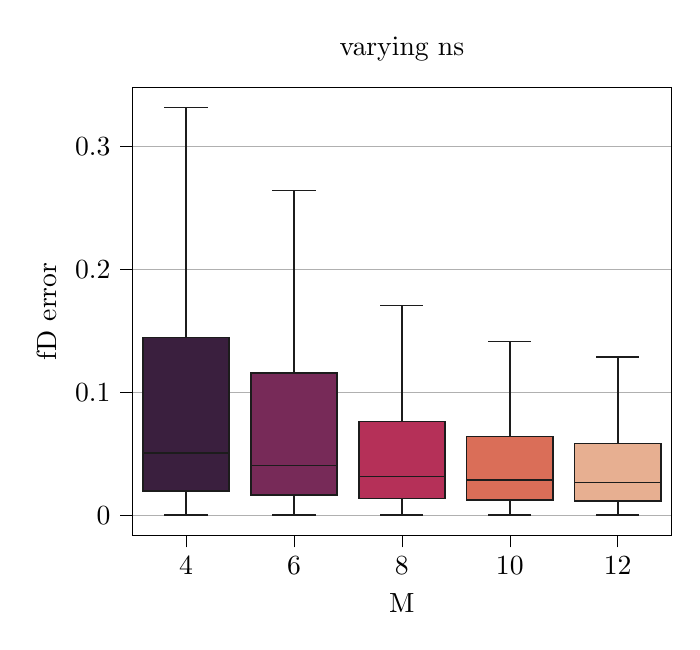
\begin{tikzpicture}

\definecolor{black28}{RGB}{28,28,28}
\definecolor{brown1814888}{RGB}{181,48,88}
\definecolor{burlywood231175145}{RGB}{231,175,145}
\definecolor{darkgray176}{RGB}{176,176,176}
\definecolor{darkslategray583162}{RGB}{58,31,62}
\definecolor{indianred21811088}{RGB}{218,110,88}
\definecolor{purple1194288}{RGB}{119,42,88}

\begin{axis}[
tick align=outside,
tick pos=left,
title={varying ns},
x grid style={darkgray176},
xlabel={M},
xmin=-0.5, xmax=4.5,
xtick style={color=black},
xtick={0,1,2,3,4},
xticklabels={4,6,8,10,12},
y grid style={darkgray176},
ylabel={fD error},
ymajorgrids,
ymin=-0.0165768972852393, ymax=0.348146454100132,
ytick style={color=black}
]
\path [draw=black28, fill=darkslategray583162, semithick]
(axis cs:-0.4,0.0193543184352735)
--(axis cs:0.4,0.0193543184352735)
--(axis cs:0.4,0.144464637100585)
--(axis cs:-0.4,0.144464637100585)
--(axis cs:-0.4,0.0193543184352735)
--cycle;
\path [draw=black28, fill=purple1194288, semithick]
(axis cs:0.6,0.0162046712851387)
--(axis cs:1.4,0.0162046712851387)
--(axis cs:1.4,0.115406443973326)
--(axis cs:0.6,0.115406443973326)
--(axis cs:0.6,0.0162046712851387)
--cycle;
\path [draw=black28, fill=brown1814888, semithick]
(axis cs:1.6,0.0133694158764787)
--(axis cs:2.4,0.0133694158764787)
--(axis cs:2.4,0.0762676105468789)
--(axis cs:1.6,0.0762676105468789)
--(axis cs:1.6,0.0133694158764787)
--cycle;
\path [draw=black28, fill=indianred21811088, semithick]
(axis cs:2.6,0.0121046108354281)
--(axis cs:3.4,0.0121046108354281)
--(axis cs:3.4,0.0638453728325134)
--(axis cs:2.6,0.0638453728325134)
--(axis cs:2.6,0.0121046108354281)
--cycle;
\path [draw=black28, fill=burlywood231175145, semithick]
(axis cs:3.6,0.0115461128081241)
--(axis cs:4.4,0.0115461128081241)
--(axis cs:4.4,0.0583108481537774)
--(axis cs:3.6,0.0583108481537774)
--(axis cs:3.6,0.0115461128081241)
--cycle;
\addplot [semithick, black28]
table {%
0 0.0193543184352735
0 1.09021120839947e-05
};
\addplot [semithick, black28]
table {%
0 0.144464637100585
0 0.331568119946251
};
\addplot [semithick, black28]
table {%
-0.2 1.09021120839947e-05
0.2 1.09021120839947e-05
};
\addplot [semithick, black28]
table {%
-0.2 0.331568119946251
0.2 0.331568119946251
};
\addplot [semithick, black28]
table {%
1 0.0162046712851387
1 2.82780164952178e-06
};
\addplot [semithick, black28]
table {%
1 0.115406443973326
1 0.264057764007141
};
\addplot [semithick, black28]
table {%
0.8 2.82780164952178e-06
1.2 2.82780164952178e-06
};
\addplot [semithick, black28]
table {%
0.8 0.264057764007141
1.2 0.264057764007141
};
\addplot [semithick, black28]
table {%
2 0.0133694158764787
2 1.98912610489113e-06
};
\addplot [semithick, black28]
table {%
2 0.0762676105468789
2 0.170513765344891
};
\addplot [semithick, black28]
table {%
1.8 1.98912610489113e-06
2.2 1.98912610489113e-06
};
\addplot [semithick, black28]
table {%
1.8 0.170513765344891
2.2 0.170513765344891
};
\addplot [semithick, black28]
table {%
3 0.0121046108354281
3 1.43686864117041e-06
};
\addplot [semithick, black28]
table {%
3 0.0638453728325134
3 0.141094555398332
};
\addplot [semithick, black28]
table {%
2.8 1.43686864117041e-06
3.2 1.43686864117041e-06
};
\addplot [semithick, black28]
table {%
2.8 0.141094555398332
3.2 0.141094555398332
};
\addplot [semithick, black28]
table {%
4 0.0115461128081241
4 6.87151500269572e-06
};
\addplot [semithick, black28]
table {%
4 0.0583108481537774
4 0.128343870053369
};
\addplot [semithick, black28]
table {%
3.8 6.87151500269572e-06
4.2 6.87151500269572e-06
};
\addplot [semithick, black28]
table {%
3.8 0.128343870053369
4.2 0.128343870053369
};
\addplot [semithick, black28]
table {%
-0.4 0.0503643210614667
0.4 0.0503643210614667
};
\addplot [semithick, black28]
table {%
0.6 0.0402655103311918
1.4 0.0402655103311918
};
\addplot [semithick, black28]
table {%
1.6 0.0315110146142871
2.4 0.0315110146142871
};
\addplot [semithick, black28]
table {%
2.6 0.0284246627182228
3.4 0.0284246627182228
};
\addplot [semithick, black28]
table {%
3.6 0.0264928241571053
4.4 0.0264928241571053
};
\end{axis}

\end{tikzpicture}
